\documentclass[10pt,addpoints]{exam}
\usepackage[utf8]{inputenc}
\usepackage[spanish,es-noshorthands]{babel}
\usepackage{hyperref}
\usepackage{amsmath}
\usepackage{amsfonts}
\usepackage{amssymb}
\usepackage{graphicx}
\usepackage{tikz,pgf}
\usepackage{multicol}
\usepackage[papersize={5.5in,8.5in},top=.7cm,bottom=.7cm,left=.7cm,right=.7cm]{geometry}
%\printanswers
\begin{document}
\title{\begin{minipage}{.2\textwidth}
        
\includegraphics[height=1.75cm]{Images/logo-colegio.png}
       \end{minipage}
\begin{minipage}{.55\textwidth}
 \begin{center}
Prueba Formativa\\Probabilidad $11^{\circ}$
\end{center}
\end{minipage}
\begin{minipage}{.2\textwidth}

\includegraphics[height=1.75cm]{Images/logo-sed.png} 
\end{minipage}
}
\author{Germ\'{a}n Avendaño Ram\'{i}rez\thanks{Lic. Mat. U.D., M.Sc. U.N.}}
\date{mayo de 2016}
\maketitle
\begin{center}
\fbox{\fbox{\parbox{4.8in}{\centering
\textit{No raye ni dañe este material. Puede usar una hoja en blanco para hacer operaciones}}}}
\end{center}
\section*{Cuestionario}
RESPONDA LAS PREGUNTAS \ref{q03}--\ref{q04} DE ACUERDO CON LA SIGUIENTE INFORMACIÓN
Una empresa ha hecho un estudio para determinar qué tan conocido es el producto que ofrece. Para este estudio realizaron encuestas dividiendo la población encuestada en tres grupos. Los resultados fueron los siguientes:
\begin{center}
\begin{tabular}{|c|p{1.85cm}|p{4cm}|p{3cm}|}
\hline 
Grupo & Total de personas encuestadas & Cantidad de personas que conocen que existe el producto pero no lo usan & Cantidad de personas que conocen y usan el producto \\ 
\hline 
I & \hspace*{.5cm}200 & \hspace*{1.5cm}110 & \hspace*{1cm}70 \\ 
\hline 
II & \hspace*{.5cm}500 & \hspace*{1.5cm}250 & \hspace*{1cm}220 \\ 
\hline 
III & \hspace*{.5cm}150 & \hspace*{1.5cm}120 & \hspace*{1cm}20 \\ 
\hline 
\end{tabular} 
\end{center}
\begin{questions}
\question \label{q03}
Una persona que lee esta información, asegura que en el grupo III se conoce más el producto, que en el grupo I. ¿Estaría usted de acuerdo con esto?
\begin{choices}
\choice no, porque la suma de la cantidad de personas que conocen que existe el producto y las que usan el producto, es mayor en el grupo I que en el III
\choice si, porque la cantidad de personas que conocen que existe el producto pero no lo usan es mayor en el grupo III que en el grupo I
\choice no, porque la cantidad de personas que conocen el producto en el grupo I corresponde al 21\% del total, mientras que en el grupo III corresponde al 16\%
\CorrectChoice si, porque la cantidad de personas que conocen el producto en el grupo III corresponde aproximadamente al 93\%, mientras que en el grupo I corresponde al 90\%
\end{choices}
\question \label{q04} Según las expectativas de la empresa, se fijó que el producto permanecería en el mercado si el 60\% de la población hace uso de él. A partir de los resultados del estudio es más probable que
\begin{choices}
\choice el producto continúe en el mercado, porque en todos los grupos la cantidad de personas que no usan el producto es menor que la cantidad de los que lo usan.
\CorrectChoice el producto no continúe en el mercado, porque sólo 31 de cada 85 personas encuestadas usan el producto.
\choice el producto continúe en el mercado, porque sólo 6 de cada 85 personas encuesta-
das no conocen el producto.
\choice el producto no continúe en el mercado, porque el porcentaje de encuestados en el
grupo III que usa el producto es aproximadamente el 2,3\% de los encuestados.
\end{choices}
\uplevel{Responda las preguntas \ref{q01}--\ref{q02} con base en la siguiente información}

A la casa que comparten cinco jóvenes ha llegado la factura de cobro del servicio de energía correspondiente al consumo del mes de septiembre. Entre la información que aparece en la factura 
se encuentra la siguiente:
\begin{center}
\begin{tabular}{lr@{}l}
consumo promedio últimos seis meses en KWh & 104 & \\ 
consumo en (KWh) & 110 & \\ 
valor (/KWh) & 175, & 0952 \\ 
costo de consumo & 19\,260 & \\ 
menos subsidio & --7\,704 & \\ 
valor neto por consumo & 11\,556 & \\ 
ajuste decena & 4 & \\ 
total a pagar & 11\,560 &
\end{tabular}
\end{center}

Uno de los jóvenes ha decidido mostrar a sus compañeros la siguiente representación gráfica de la información proporcionada en la factura
\begin{center}
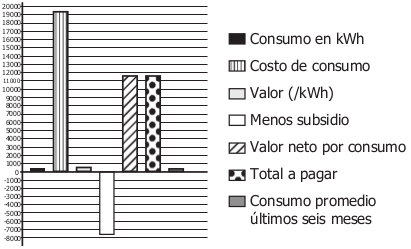
\includegraphics[scale=.7]{Images/consumo.png} 
\end{center}
\question \label{q01}
Uno de los jóvenes, al analizar la gráfica, hace la observación de que no debe presentarse así, puesto que
\begin{choices}
\choice en la gráfica se relaciona correctamente la información de la factura, sin embargo para facilitar la lectura sería más conveniente organizar las barras por tamaño.
\choice la gráfica está mal construida porque la barra que indica subsidio no debería corresponder a un valor negativo ya que es un ahorro y no un gasto.
\CorrectChoice no es posible relacionar todos los datos de la factura en una gráfica como ésta, porque la escala numérica no puede asociarse a pesos y kWh simultáneamente.
\choice no es posible que la gráfica sea correcta porque el total a pagar no puede ser menor que el costo del consumo.
\end{choices}
\question  \label{q02} Los jóvenes están preocupados porque el consumo promedio relacionado en la factura, aumentó en 6 kWh respecto al relacionado en el mes de agosto. Discuten porque según ellos deben pagar 36 kWh más que en el mes de agosto. Esto no debería ser razón de discusión pues
\begin{choices}
\choice el aumento en el consumo realmente fue de 6 kWh respecto al mes de marzo.
\choice el dato proporcionado corresponde a un promedio y por tanto no es posible comparar el consumo de septiembre con el de ninguno de los seis meses anteriores.
\choice el consumo sí aumentó en 36 kWh, pero respecto al consumo de abril y no al de agosto.
\CorrectChoice el consumo sí aumentó en 36 kWh, pero respecto al consumo de marzo y no al de agosto.
\end{choices}
\question \label{q05} Una empresa de transporte cuenta con vehículos de tres modelos distintos para cubrir tres rutas en una ciudad durante los días lunes, miércoles y viernes. En la tabla 1 se muestra el número de vehículos de cada modelo que se tiene para cada ruta y en la tabla 2 se muestra el consumo diario de gasolina (medido en galones) de cada modelo.
\begin{center}
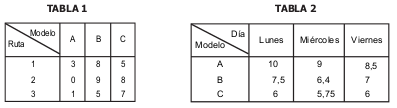
\includegraphics[scale=.8]{Images/tablas.png} 
\end{center}
La tabla que representa la información sobre el consumo de gasolina por ruta durante los días de recorrido es:
\begin{center}
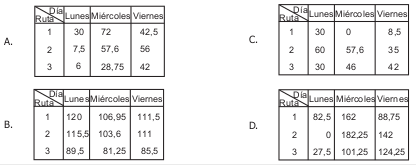
\includegraphics[scale=.8]{Images/tablas01.png} 
\end{center}
\question \label{q06} En una institución escolar, de un grupo de 10 estudiantes conformado por 6 hombres y 4 mujeres, se van a elegir por votación:
\begin{itemize}
\item 1 personero
\item 1 representante al consejo directivo
\item 3 representantes al consejo estudiantil (para ocupar los cargos de presidente, secretario y tesorero)
\end{itemize}
La probabilidad de que los estudiantes elegidos sean 2 hombres y 3 mujeres es igual
a la probabilidad de que los elegidos sean
\begin{choices}
\CorrectChoice 4 hombres y 1 mujer
\choice 1 hombre y 4 mujeres
\choice 3 hombres y 2 mujeres
\choice 5 hombres y ninguna mujer
\end{choices}
\question \label{q07} Al realizar el diseño de un edificio, el arquitecto propone que el ascensor sea panorámico; es decir que tenga total visibilidad hacia el exterior desde sus caras laterales, excepto la trasera, como se muestra en el dibujo.
\begin{center}
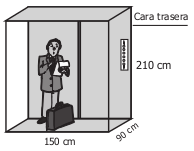
\includegraphics[scale=.8]{Images/Pantallazo-40.png} 
\end{center}
La capacidad del ascensor que se construye es de 560 kilogramos (kg). Si lo usan simultáneamente 6 adultos y 4 niños y el peso promedio de los adultos es 70 kg, el peso promedio máximo de los niños para que no se supere la capacidad del ascensor es

\begin{oneparchoices}
\choice 25 kg
\choice 30 kg
\CorrectChoice 35 kg
\choice 40 kg
\end{oneparchoices}
%\choice[1] Nunca
%\end{oneparchoices}
%\answerline
\end{questions}
%cuadro de puntajes
%\begin{center}
%\gradetable[h][pages]
%\end{center}
\end{document}